\scanpage{162}
\margin{\figure{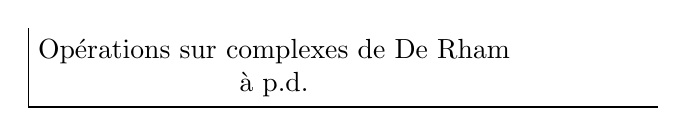
\begin{tikzpicture}\node[align=center,anchor=south west] at (0,0) {Opérations sur complexes de De Rham\\à p.d.};\draw (0,1)--(0,0)--(8,0);\end{tikzpicture}}}
\deleted{Proposition}
\uline{Théorème} Soient $(S,S^+,t)$ et $(S',S'^+,t')$ deux anneaux (comm.) à idéal à p.d. et élément marqué dedans
(\uline{\unsure{ps}} $S^+=(t)_{\mathrm{p.d.}}$, $S'^+=(t')_{\mathrm{pd}}$)
d'où
\[
 \begin{array}{ccc}\mathcal A(S,S^+,t)_*&\text{et}&
 \mathcal A'(S',S'^+,t')_*\\
 \Vert&&\Vert\\
 \mathcal A_S&&\mathcal A_{S'}\end{array},
\]
qu'on considère comme anneaux différentiels \unsure{$\tfrac12$|$k$}-simpliciaux
(faisant abstraction de leurs structures graduée, filtrée, à p.d., et de $S$ et $S'$ algèbres\ldots).
Alors les hom \inserted{$\varphi$} de tels anneaux \inserted{différentiels \unsure{$\tfrac12$|$k$}-simpliciaux} correspondent biunivoquement aux systèmes $(\varphi_0,A'_{\deleted{1}},(B'_i)_{i\geq1})$, où
\[
 \left\{\begin{aligned}
 &\varphi_0:S\mathbin{\text{---}}S'\quad\text{un hom d'anneaux}\\
 &A'_{\deleted{1}}\in S'\{X_0\}^{++}=\operatorname{Ker}(\alpha_{S'}:S'\{X_0\}\mathbin{\text{---}}S';\ \alpha(X_0^{(i)})=0\quad\forall i\geq1)\\
 &B'_i\in S'\{X_0\}
 \end{aligned}\right.
\]
sont donnés en fonction de $\varphi$ par
\[
 \left\{\begin{aligned}
 &\varphi_0=\text{composante de degré }0\text{ de }\varphi,\\
 &A'_{\deleted{1}}=\unsure{K_0|\pi_0}\varphi_1(X_0)\\
 &B'_i=\unsure{K_1|\pi_1}\varphi_1(X_0^{(i)})
 \end{aligned}\right.
\]
\diagram{\begin{tikzcd}
 \varphi_0:(\mathcal A_S)_0\arrow[r,dash]\arrow[d,equal]&(\mathcal A_{S'})_0\arrow[d,equal]\\
 S&S'
\end{tikzcd}}
\diagram{\begin{tikzcd}
 \varphi_1:S\{X_0\}\deleted{[dX_0]}\arrow[r]\arrow[d,equal]&S'\{X_0\}[dX_0]\arrow[d,equal]\\
 (\mathcal A_S)_1&(\mathcal A_{S'})_1
\end{tikzcd}}
$\unsure{K_0|\pi_0},\unsure{K_1|\pi_1}$ les projections sur les composantes de degré $0$ resp. $1$

\inserted{$(\varphi_0,A'_1,B'_i\ (i\geq1))$}
satisfaisant aux conditions
\[
 \left\{\begin{aligned}
 1)\quad&\deleted{\unsure{f_i}}\ \varphi_0(t^{(i)})=\varphi_0(t)^{(i)}
 &&\text{i.e. }\varphi_0\text{ commute aux p.d. sur }(t)_{\mathrm{pd}}\ (!)\\
 2)\quad&\beta_{S'}(A'_{\deleted{1}})=\varphi_0(t)
 &&\text{i.e. si }A'_{\deleted{1}}=\sum_{j\geq1}a'_{\deleted{1}j}X_0^{(j)},\text{ on a}\\
 &\sum_{j\geq1}a'_j t'^{(j)}=\varphi_0(t)\\
 3)\quad&(2^{\unsure{i|*}}B'_i)J'=0\ \deleted{\unsure{(A',B'_j)}}
 &&\forall i\geq1,
 \end{aligned}\right.
\]
où $J'$ est l'idéal de $S'$ engendré par les coeff. $a'_j$ de $A'$ et les coeff. $b'_{jh}$ des
\[
 B'_j=\sum_{h\geq0}b'_{jh}X_0^{(h)}.
\]
\margin{\uline{NB} dans la suite, supprimer l'indice $1$ à $A'_1$}
[\uline{NB} Si $\varphi_0(t)$ est \deleted{un élément} \inserted{\unsure{élémt} régulier} de $S'$ alors en vertu de \unsure{(2)} $J$ contient un élément régulier et les relations \unsure{(3)}
\margin{TSVP $\longrightarrow$}
\margin{161}
